\documentclass[11pt, spanish, a4paper, twopage]{article}

% Versión 1.er cuat 2021 Víctor Bettachini < vbettachini@unlam.edu.ar >

\usepackage[T1]{fontenc}
\usepackage[utf8]{inputenc}

\usepackage[spanish, es-tabla]{babel}
\def\spanishoptions{argentina} % Was macht dass?
% \usepackage{babelbib}
% \selectbiblanguage{spanish}
% \addto\shorthandsspanish{\spanishdeactivate{~<>}}

\usepackage{graphicx}
\graphicspath{{./figuras/}{../LaTeX/}}
% \usepackage{float}

\usepackage[arrowdel]{physics}
\newcommand{\pvec}[1]{\vec{#1}\mkern2mu\vphantom{#1}}
% \usepackage{units}
\usepackage[separate-uncertainty= true, multi-part-units= single, range-units= single, range-phrase= {~a~}, locale= FR]{siunitx}
\usepackage{isotope} % $\isotope[A][Z]{X}\to\isotope[A-4][Z-2]{Y}+\isotope[4][2]{\alpha}

\usepackage{tasks}
\usepackage[inline]{enumitem}
% \usepackage{enumerate}

\usepackage{hyperref}

% \usepackage{amsmath}
% \usepackage{amstext}
% \usepackage{amssymb}

\usepackage{tikz}
\usepackage{tikz-dimline}
\usetikzlibrary{calc}
% \usetikzlibrary{math}
\usetikzlibrary{arrows.meta}
\usetikzlibrary{snakes}
\usetikzlibrary{decorations}
\usetikzlibrary{decorations.pathmorphing}
\usetikzlibrary{patterns}

\usepackage[hmargin=1cm,vmargin=3cm, top= 0.75cm,nohead]{geometry}

\usepackage{lastpage}
\usepackage{fancyhdr}
\pagestyle{fancyplain}
\fancyhf{}
\setlength\headheight{28.7pt} 
\fancyhead[LE, LO]{\textbf{Mecánica General} }
\fancyhead[RE, RO]{\href{https://ingenieria.unlam.edu.ar/}{$\vcenter{\hbox{
\includegraphics[height=1cm]{ambos.pdf}}}$}}
\fancyfoot{\href{https://creativecommons.org/licenses/by-nc-sa/4.0/deed.es_ES}{$\vcenter{\hbox{
\includegraphics[height=0.4cm]{by-nc-sa_80x15.pdf}}}$} \href{https://ingenieria.unlam.edu.ar/}{DIIT - UNLaM}}
\fancyfoot[C]{ {\tiny Actualizado al \today} }
\fancyfoot[RO, LE]{Pág. \thepage/\pageref{LastPage}}
\renewcommand{\headrulewidth}{0pt}
\renewcommand{\footrulewidth}{0pt}



\begin{document}
\begin{center}
  % \textsc{\large Mecánica general}\\
  \textsc{\large Coordenadas generalizadas | Ligaduras | Energía}
\end{center}

\noindent
%De poder resolver estos problemas en forma autónoma puede asumir que adquirió los conocimientos mínimos sobre los temas abordados en la semana.
%No dude en consultar a docentes y compañeros si no puede terminarlos.
Los problemas marcados con (*) tienen alguna dificultad adicional, no dude en consultar.
\begin{enumerate}


%\item \begin{minipage}[t][3cm]{0.7\textwidth}
%\textbf{Péndulo ideal rígido} [Marion ex. 7.2]\\
%Escriba y resuelva la ecuación que describe la dinámica de un péndulo de longitud $\ell$ en presencia de un campo gravitatorio de constante $g$. Discuta todas las aproximaciones que realiza.
%\end{minipage}
%\begin{minipage}[c][1cm][t]{0.25\textwidth}
%%	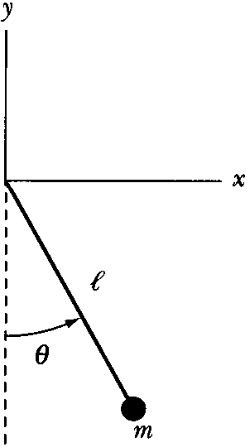
\includegraphics[width=0.75\textwidth]{marion_fig7_1}
%%	\includegraphics[width=\textwidth]{\detokenize{pénduloHorizontal}}
%	\begin{tikzpicture}
%	%\begin{tikzpicture}[scale= 1.2]
%  	\draw [arrows=- triangle 45] (-1,2) -> (-1,1) node [above=15, right=2] {\(\vec{g}\)}; % g vertical
%		\draw [ultra thick] (-1.5,3) -- (2.5,3);
%		\fill [pattern = north east lines] (-1.5,3) rectangle (2.5,3.2); % techo
%		\draw [dashed] (0,3) -- (0,0);	% vertical
%		\draw [thick] (0,3) -- +(-60:3) node[midway,above,right=2] {\(\ell\)};	% inclinada +:relativa, -60 grados, longitud 3
%		% \draw [thick] (0,3) -- +(-60:3) node[midway,above,sloped] {\(l\)};	% inclinada +:relativa, -60 grados, longitud 3
%    \fill (0,3)+(-60:3) circle [radius=0.25] node [text=white] { \( \mathrm{m} \) }; % masa izq
%    \draw [thin, arrows=- triangle 45] (0,.4) -> (1.25,.4) node [midway, above] {\( \psi \)}; % desplazamiento horizontal
%    % \draw [thin, arrows=- triangle 45] (0,.4) -> (1.25,.4) node [above=8, left=8] {\( \psi \)}; % desplazamiento horizontal
%		\draw [thin, arrows=- triangle 45] (0,0) arc [start angle=-90, end angle=-65, radius=3] node [below=12, left=8] {\( \varphi \)};
%	\end{tikzpicture}
%\end{minipage}




\item \begin{minipage}[t][4cm]{0.7\textwidth}
\textbf{Péndulo con punto de suspensión libre} [Landau \S5 ej. 2]\\
Un péndulo oscila en un plano de masa \(m_2\) cuyo punto de suspensión, de masa \(m_1\), puede desplazarse sobre una recta horizontal.
\begin{enumerate}
	\item Escriba la energía cinética, \(T\) y potencial, \(V\), en función de las coordenadas generalizadas sugeridas por las figura.
	\item Verifique que al fijar la masa \(m_1\) recupera las expresiones de \(T\) y \(V\) de un péndulo simple.
\end{enumerate}
\end{minipage}
\begin{minipage}[c][1cm][t]{0.3\textwidth}
        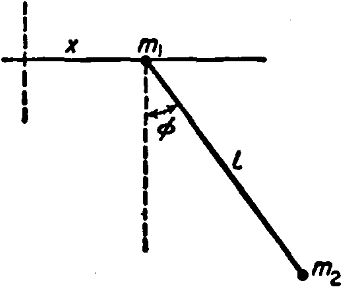
\includegraphics[width=0.75\textwidth]{landauS52_fig2.png}
\end{minipage}



\item \begin{minipage}[t][4cm]{0.7\textwidth}
\textbf{Péndulo doble} [Landau \S5 ej. 1]\\
Un péndulo doble oscila en un plano en función de las coordenadas generalizadas sugeridas por las figura.
\begin{enumerate}
	\item Calcule la energía cinética, \(T\) y potencial, \(V\).
	\item Verifique que recupera \(T\) y \(V\) de un péndulo simple de asumir \(m_1=0\), \(\varphi_1 = \varphi_2 = \varphi\) y \(\ell_1 = \ell_2 = \frac{l}{2}\).
\end{enumerate}
Ayuda: \( \cos(\alpha \pm \beta) = \cos{ \alpha} \cos{ \beta \mp \sin \alpha} \sin{ \beta } \)
\end{minipage}
\begin{minipage}[c][0.5cm][t]{0.3\textwidth}
	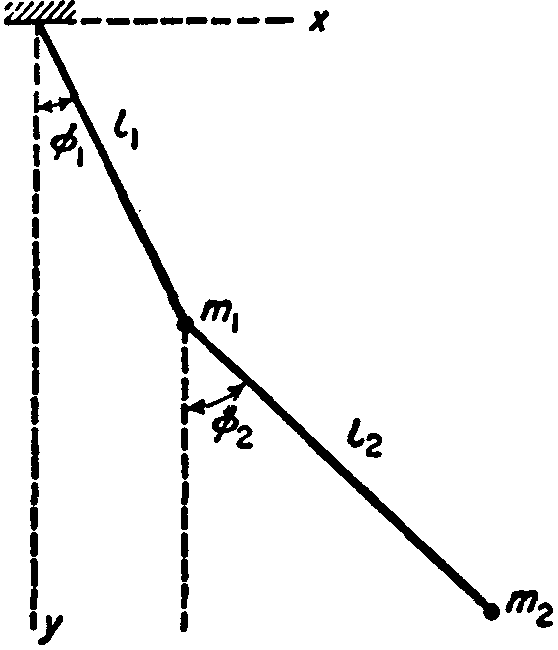
\includegraphics[width=0.75\textwidth]{landauS52_fig1.png}
\end{minipage}



\item \begin{minipage}[t][7cm]{0.5\textwidth}
(*) \textbf{Péndulo con punto de suspensión en rotación} [Marion (e) ex. 7.5] [Landau \S5 ej. 3]\\
El punto de suspensión de un péndulo que se mueve en el plano plano se desplaza en un círculo vertical de radio \(a\) con una frecuencia \(\omega\).

Calcule la energía cinética, \(T\) y potencial, \(V\).
\end{minipage}
	\begin{minipage}[c][3cm][t]{0.5\textwidth}
	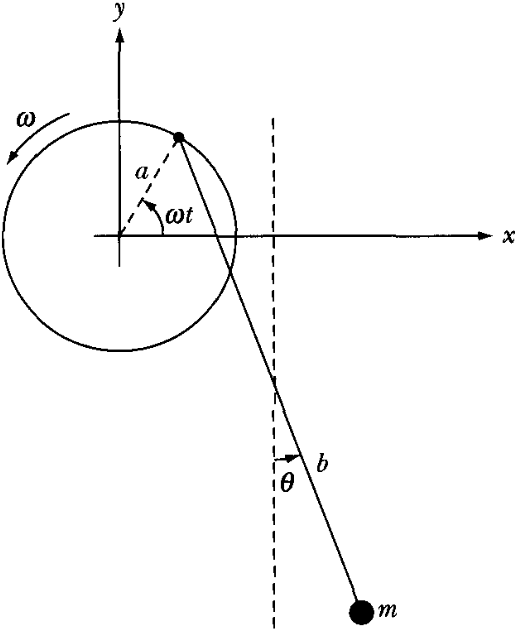
\includegraphics[width=0.75\textwidth]{marion_fig7_3.png}
	% 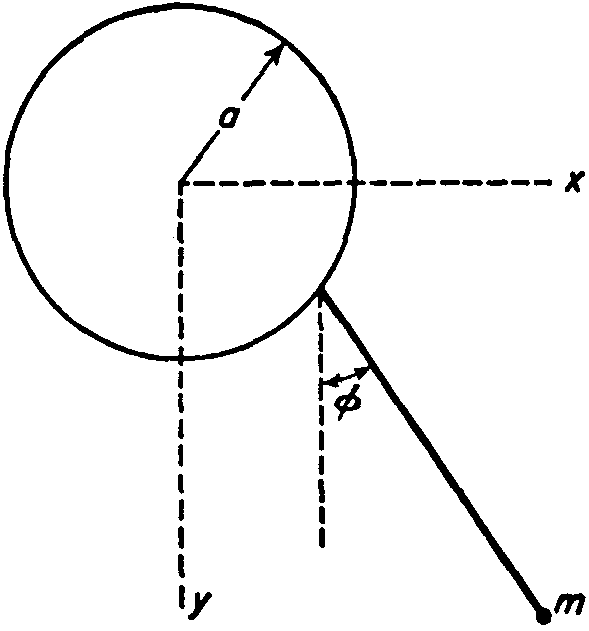
\includegraphics[width=0.75\textwidth]{landauS52_fig3.png}
\end{minipage}



\item \begin{minipage}[t][4.5cm]{0.65\textwidth}
(*) \textbf{Pesas acopladas rotando en torno a eje} [Landau \S5 ej. 4]\\
La partícula con \(m_2\) se desplaza sobre un eje vertical, y todo el sistema gira con una velocidad angular constante \(\Omega\) en torno a ese eje.

Calcule la energía cinética, \(T\) y potencial, \(V\).
\end{minipage}
	\begin{minipage}[c][5cm][t]{0.35\textwidth}
	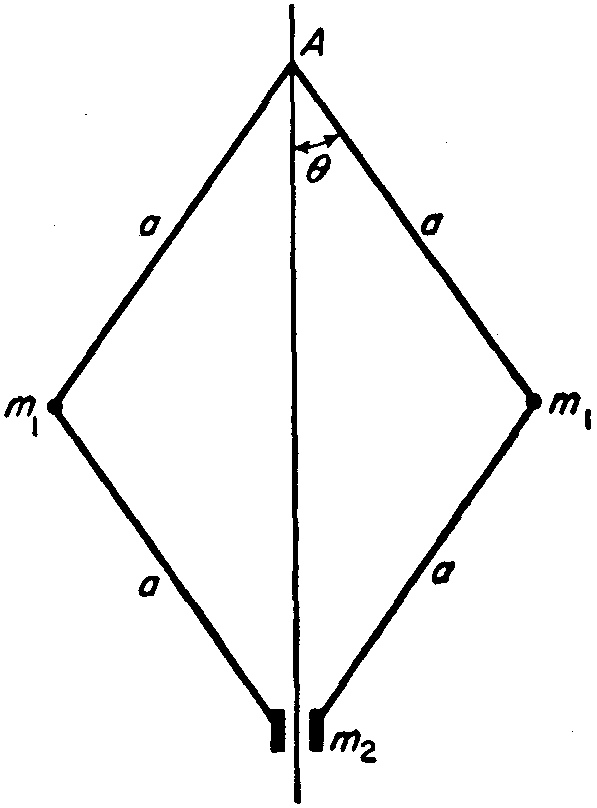
\includegraphics[width=0.75\textwidth]{landauS52_fig4.png}
\end{minipage}



\end{enumerate}
\end{document}
